% Options for packages loaded elsewhere
\PassOptionsToPackage{unicode}{hyperref}
\PassOptionsToPackage{hyphens}{url}
%
\documentclass[
  ignorenonframetext,
  aspectratio=169,
  c]{beamer}
\usepackage{pgfpages}
\setbeamertemplate{caption}[numbered]
\setbeamertemplate{caption label separator}{: }
\setbeamercolor{caption name}{fg=normal text.fg}
\beamertemplatenavigationsymbolshorizontal
% Prevent slide breaks in the middle of a paragraph
\widowpenalties 1 10000
\raggedbottom
\setbeamertemplate{part page}{
  \centering
  \begin{beamercolorbox}[sep=16pt,center]{part title}
    \usebeamerfont{part title}\insertpart\par
  \end{beamercolorbox}
}
\setbeamertemplate{section page}{
  \centering
  \begin{beamercolorbox}[sep=12pt,center]{part title}
    \usebeamerfont{section title}\insertsection\par
  \end{beamercolorbox}
}
\setbeamertemplate{subsection page}{
  \centering
  \begin{beamercolorbox}[sep=8pt,center]{part title}
    \usebeamerfont{subsection title}\insertsubsection\par
  \end{beamercolorbox}
}
\AtBeginPart{
  \frame{\partpage}
}
\AtBeginSection{
  \ifbibliography
  \else
    \frame{\sectionpage}
  \fi
}
\AtBeginSubsection{
  \frame{\subsectionpage}
}

\usepackage{amsmath,amssymb}
\usepackage{iftex}
\ifPDFTeX
  \usepackage[T1]{fontenc}
  \usepackage[utf8]{inputenc}
  \usepackage{textcomp} % provide euro and other symbols
\else % if luatex or xetex
  \usepackage{unicode-math}
  \defaultfontfeatures{Scale=MatchLowercase}
  \defaultfontfeatures[\rmfamily]{Ligatures=TeX,Scale=1}
\fi
\usepackage{lmodern}
\usetheme[]{Luebeck}
\usecolortheme{beaver}
\ifPDFTeX\else  
    % xetex/luatex font selection
\fi
% Use upquote if available, for straight quotes in verbatim environments
\IfFileExists{upquote.sty}{\usepackage{upquote}}{}
\IfFileExists{microtype.sty}{% use microtype if available
  \usepackage[]{microtype}
  \UseMicrotypeSet[protrusion]{basicmath} % disable protrusion for tt fonts
}{}
\makeatletter
\@ifundefined{KOMAClassName}{% if non-KOMA class
  \IfFileExists{parskip.sty}{%
    \usepackage{parskip}
  }{% else
    \setlength{\parindent}{0pt}
    \setlength{\parskip}{6pt plus 2pt minus 1pt}}
}{% if KOMA class
  \KOMAoptions{parskip=half}}
\makeatother
\usepackage{xcolor}
\newif\ifbibliography
\setlength{\emergencystretch}{3em} % prevent overfull lines
\setcounter{secnumdepth}{-\maxdimen} % remove section numbering


\providecommand{\tightlist}{%
  \setlength{\itemsep}{0pt}\setlength{\parskip}{0pt}}\usepackage{longtable,booktabs,array}
\usepackage{calc} % for calculating minipage widths
\usepackage{caption}
% Make caption package work with longtable
\makeatletter
\def\fnum@table{\tablename~\thetable}
\makeatother
\usepackage{graphicx}
\makeatletter
\def\maxwidth{\ifdim\Gin@nat@width>\linewidth\linewidth\else\Gin@nat@width\fi}
\def\maxheight{\ifdim\Gin@nat@height>\textheight\textheight\else\Gin@nat@height\fi}
\makeatother
% Scale images if necessary, so that they will not overflow the page
% margins by default, and it is still possible to overwrite the defaults
% using explicit options in \includegraphics[width, height, ...]{}
\setkeys{Gin}{width=\maxwidth,height=\maxheight,keepaspectratio}
% Set default figure placement to htbp
\makeatletter
\def\fps@figure{htbp}
\makeatother

\makeatletter
\@ifpackageloaded{caption}{}{\usepackage{caption}}
\AtBeginDocument{%
\ifdefined\contentsname
  \renewcommand*\contentsname{Table of contents}
\else
  \newcommand\contentsname{Table of contents}
\fi
\ifdefined\listfigurename
  \renewcommand*\listfigurename{List of Figures}
\else
  \newcommand\listfigurename{List of Figures}
\fi
\ifdefined\listtablename
  \renewcommand*\listtablename{List of Tables}
\else
  \newcommand\listtablename{List of Tables}
\fi
\ifdefined\figurename
  \renewcommand*\figurename{Figure}
\else
  \newcommand\figurename{Figure}
\fi
\ifdefined\tablename
  \renewcommand*\tablename{Table}
\else
  \newcommand\tablename{Table}
\fi
}
\@ifpackageloaded{float}{}{\usepackage{float}}
\floatstyle{ruled}
\@ifundefined{c@chapter}{\newfloat{codelisting}{h}{lop}}{\newfloat{codelisting}{h}{lop}[chapter]}
\floatname{codelisting}{Listing}
\newcommand*\listoflistings{\listof{codelisting}{List of Listings}}
\makeatother
\makeatletter
\makeatother
\makeatletter
\@ifpackageloaded{caption}{}{\usepackage{caption}}
\@ifpackageloaded{subcaption}{}{\usepackage{subcaption}}
\makeatother
\makeatletter
\@ifpackageloaded{sidenotes}{}{\usepackage{sidenotes}}
\@ifpackageloaded{marginnote}{}{\usepackage{marginnote}}
\makeatother
\ifLuaTeX
  \usepackage{selnolig}  % disable illegal ligatures
\fi
\usepackage{bookmark}

\IfFileExists{xurl.sty}{\usepackage{xurl}}{} % add URL line breaks if available
\urlstyle{same} % disable monospaced font for URLs
\hypersetup{
  pdftitle={Age du Faire et du Do-It-Youself (DIY)},
  pdfauthor={MdC. Fabio Cruz},
  hidelinks,
  pdfcreator={LaTeX via pandoc}}

\title{Age du Faire et du Do-It-Youself (DIY)}
\subtitle{An introduction}
\author{MdC. Fabio Cruz}
\date{2023-01-13}
\institute{Université de Lorraine \textbar{} ENSGSI}

\begin{document}
\frame{\titlepage}

\section{Planning}\label{planning}

\subsection{Planning}\label{planning-1}

\begin{frame}{Planning}
\begin{longtable}[]{@{}ll@{}}
\toprule\noalign{}
\textbf{Time} & \textbf{Activity} \\
\midrule\noalign{}
\endhead
13:45 - 14:15 & Introduction to LF2L and key concepts \\
14:15 - 15:00 & Design of the your obj \\
15:00 - 15:20 & \emph{Break} 🍏 \\
15:20 - 16:00 & Fabrication of your totem \\
16:00 - 16:45 & Documentation of FabManager \\
\bottomrule\noalign{}
\end{longtable}
\end{frame}

\subsection{Goal of the day}\label{goal-of-the-day}

\begin{frame}{Goal of the day}
\begin{columns}[T]
\begin{column}{0.48\textwidth}
\end{column}

\begin{column}{0.48\textwidth}
\end{column}
\end{columns}
\end{frame}

\section{Engineering, `Age du Faire and
DIY'}\label{engineering-age-du-faire-and-diy}

\subsection{What is the meaning of ``Engineer'' for you
?}\label{what-is-the-meaning-of-engineer-for-you}

\begin{frame}{What is the meaning of ``Engineer'' for you ?}
The word \textbf{Engineer} (Latin \emph{Ingeniator}) is derived from the
Latin words \textbf{Ingeniare} (``to contrive, devise'') and
\textbf{Ingenium} (``cleverness'').
\end{frame}

\subsection{Fab Lab and how to do (almost)
anything}\label{fab-lab-and-how-to-do-almost-anything}

\begin{frame}{Fab Lab and how to do (almost) anything}
\marginnote{\begin{footnotesize}

Source: \url{https://cba.mit.edu/classes/}

\end{footnotesize}}
\end{frame}

\subsection{Unleash your creativity in a Fab Lab. Feb
2006}\label{unleash-your-creativity-in-a-fab-lab.-feb-2006}

\begin{frame}{Unleash your creativity in a Fab Lab. Feb 2006}
Source:
https://www.ted.com/talks/neil\_gershenfeld\_unleash\_your\_creativity\_in\_a\_fab\_lab
\end{frame}

\subsection{What is a Fablab?}\label{what-is-a-fablab}

\begin{frame}{What is a Fablab?}
\begin{center}
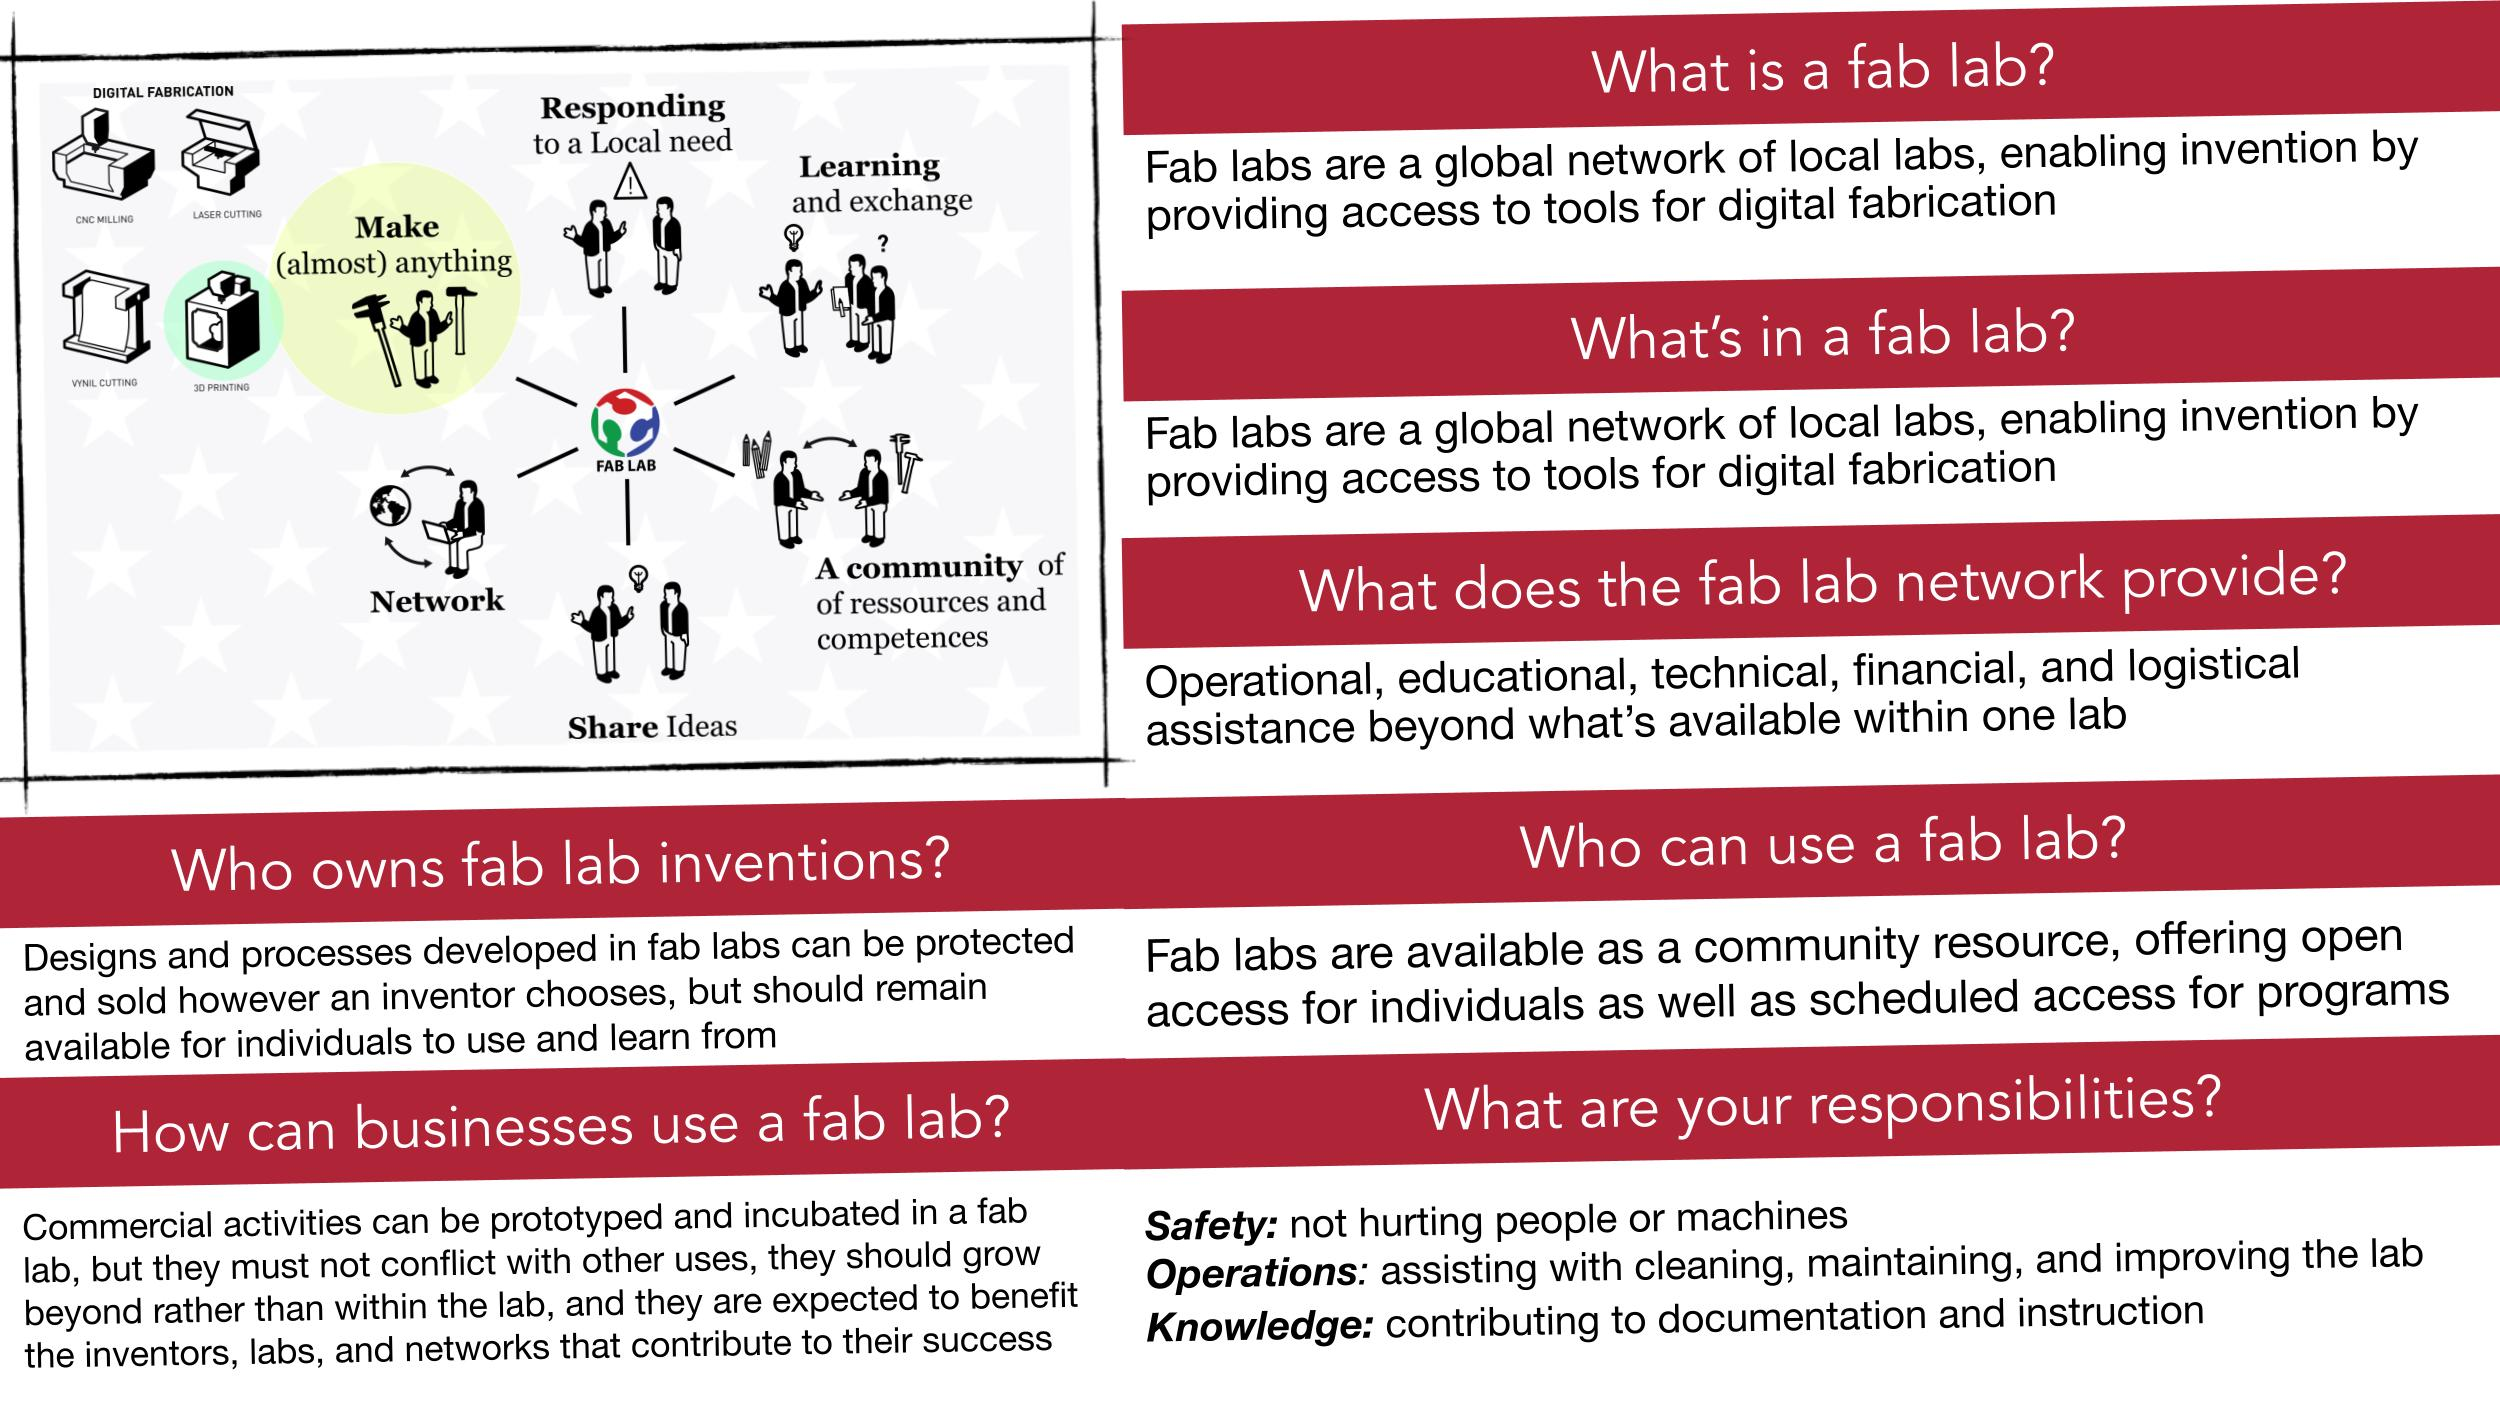
\includegraphics[width=0.9\textwidth,height=\textheight]{figures/Fablab-definition-00.jpg}
\end{center}

Source: \url{https://fab.cba.mit.edu/about/charter/}
\end{frame}

\subsection{Personal Fabrication}\label{personal-fabrication}

\begin{frame}{Personal Fabrication}
\begin{columns}[T]
\begin{column}{0.48\textwidth}
\emph{Products for a market of \textbf{one person}}
\end{column}

\begin{column}{0.48\textwidth}
\end{column}
\end{columns}
\end{frame}

\section{Lorraine Fab Living Lab}\label{lorraine-fab-living-lab}

\subsection{Lorraine Fab Living Lab}\label{lorraine-fab-living-lab-1}

\begin{frame}{Lorraine Fab Living Lab}
\begin{columns}[T]
\begin{column}{0.48\textwidth}
\begin{center}

\includegraphics[width=3.64583in,height=\textheight]{figures/LF2L-Vertical.jpg}
\end{center}

\textbf{Research platform for prospective assessment of innovative
usages}
\end{column}

\begin{column}{0.48\textwidth}
\end{column}
\end{columns}
\end{frame}

\subsection{\texorpdfstring{Materialize \emph{Citizen
Innovation}?}{Materialize Citizen Innovation?}}\label{materialize-citizen-innovation}

\begin{frame}{Materialize \emph{Citizen Innovation}?}
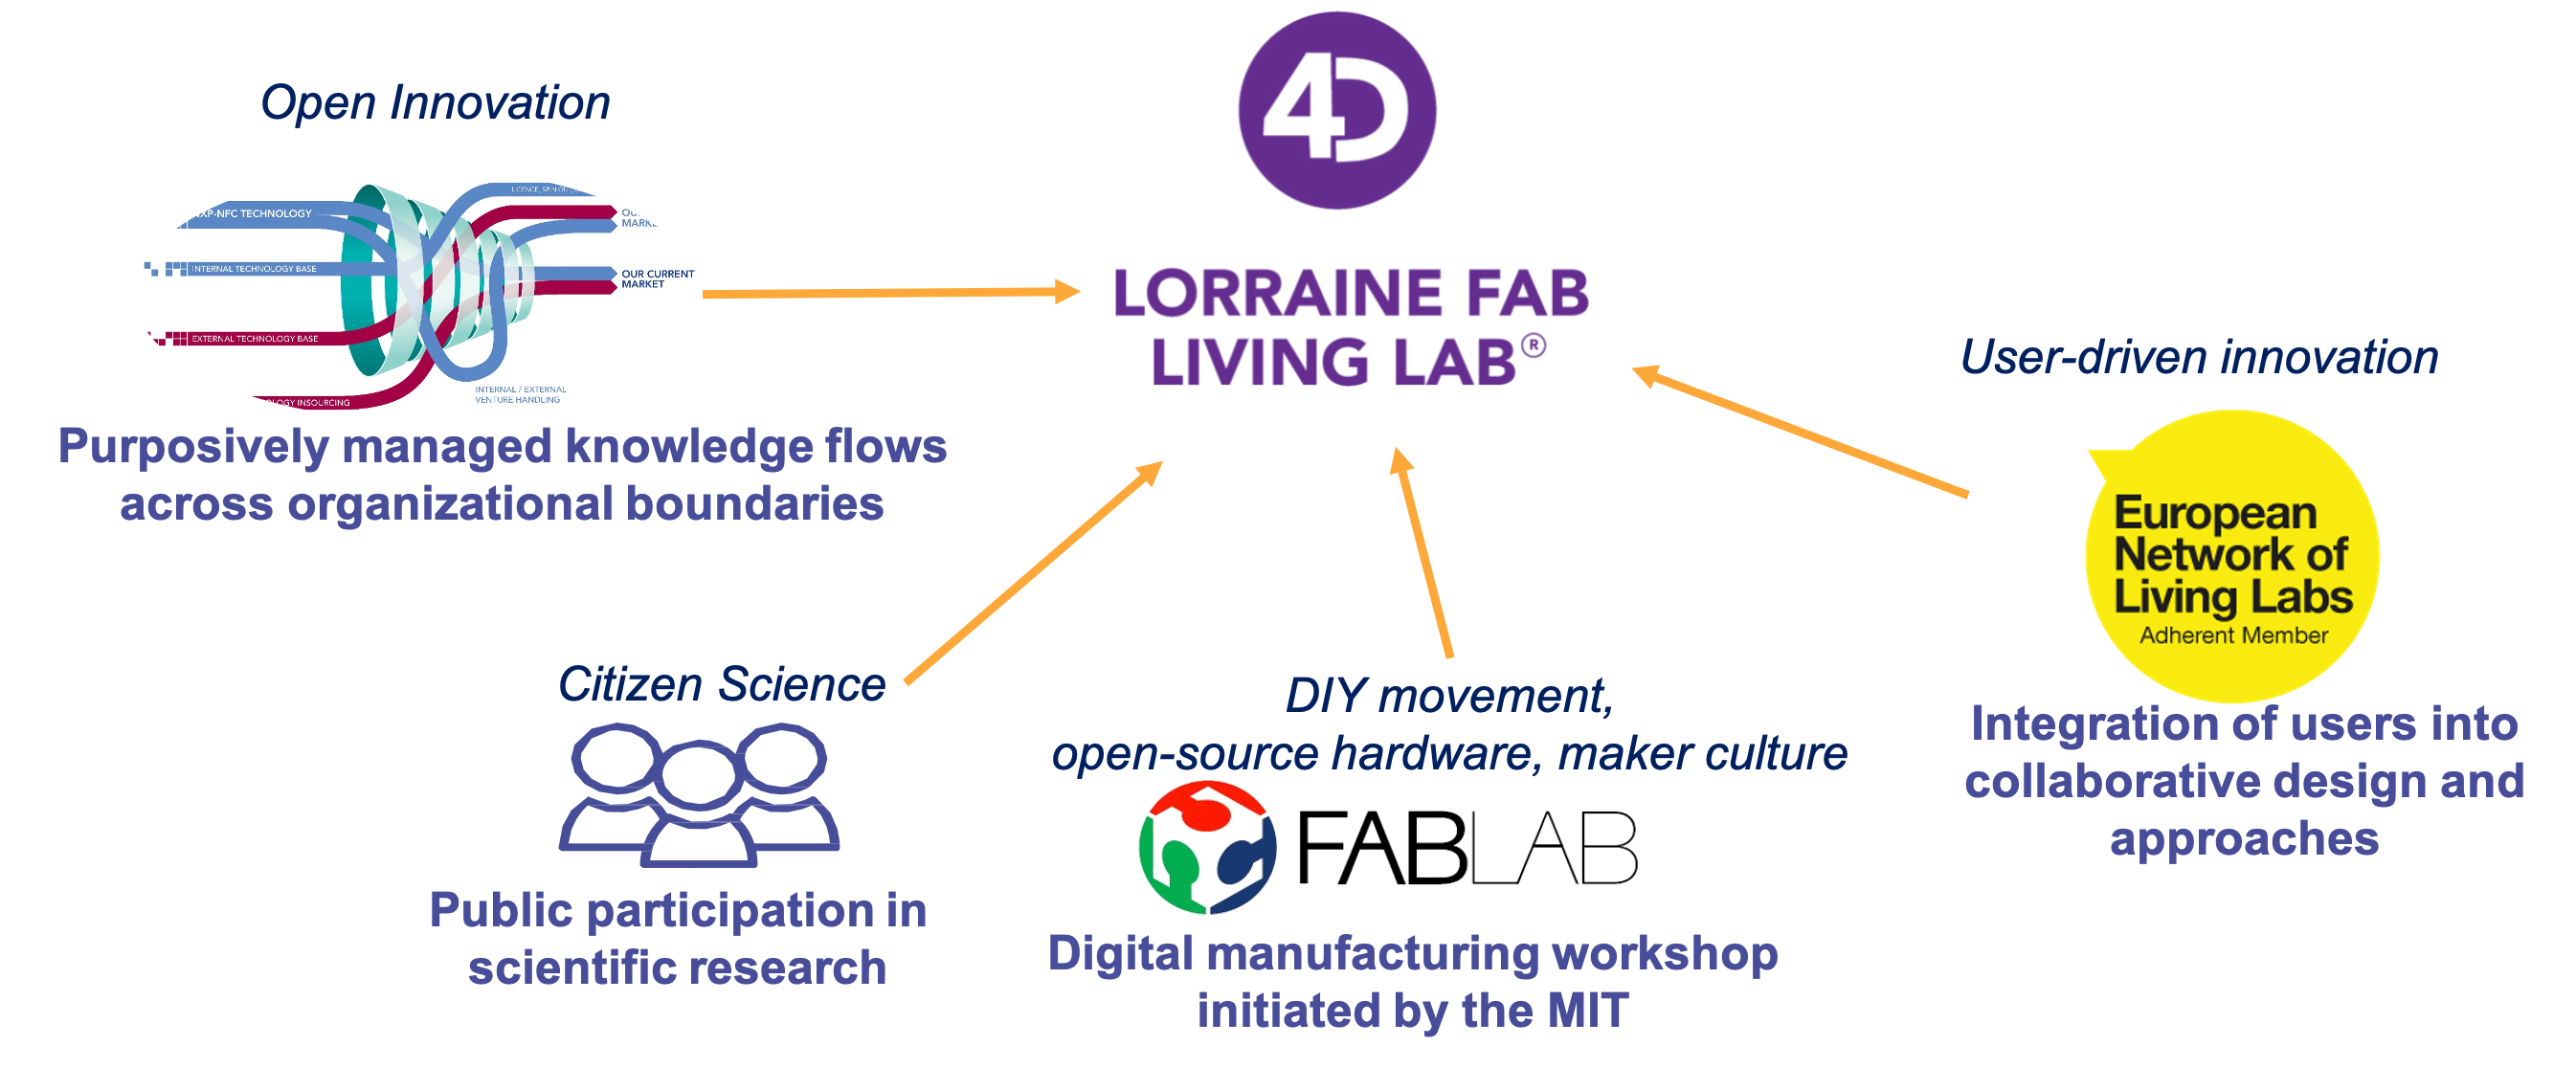
\includegraphics{figures/Materialize-Innovation-00.png}
\end{frame}

\subsection{Why Prototyping Matters ?}\label{why-prototyping-matters}

\begin{frame}{Why Prototyping Matters ?}
\textbf{``Humans are really interesting. If you show them your idea in a
prototype form, very few people will tell you what's right about it.
\emph{But everybody will tell you what's wrong with it}.''} David Kelly,
IDEO
\end{frame}

\subsection{What is Prototyping ?}\label{what-is-prototyping}

\begin{frame}{What is Prototyping ?}
\begin{quote}
``The process of creating usable artifacts at a variety of fidelities of
completion, in order to answer design questions and communicate design
ideas; with users in the context of use.''
\end{quote}
\end{frame}

\subsection{What is Prototyping ?}\label{what-is-prototyping-1}

\begin{frame}{What is Prototyping ?}
\begin{quote}
``The \textbf{process of creating} usable artifacts at a variety of
fidelities of completion, in order to answer design questions and
communicate design ideas; with users in the context of use.''
\end{quote}

\begin{center}
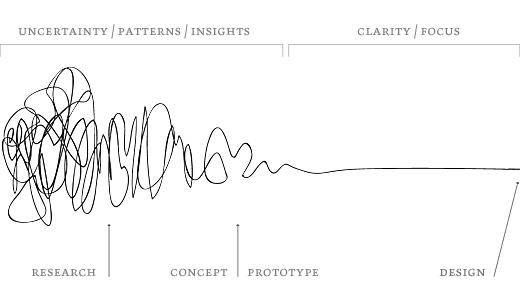
\includegraphics{figures/process-explained-1.jpg}
\end{center}
\end{frame}

\section{TP: Design a recycled totem}\label{tp-design-a-recycled-totem}



\end{document}
